\section{Requisiti soddisfatti}
Seguendo quanto definito nel \PdPv{v3.0.0-0.2} il gruppo è riuscito a soddisfare tutti i requisiti obbligatori. Arrivati a questo punto si è avviata anche la codifica delle funzionalità opzionali e desiderabili che proseguirà nel periodo successivo alla RQ. 
\subsection{Tabella del soddisfacimento dei requisiti}
\renewcommand{\arraystretch}{1.5}	 
{
\setlength\arrayrulewidth{1pt}
\begin{longtable}{C{2.5cm} C{2cm} C{3.5cm}}
		\rowcolor{coloreRosso}
		\textcolor{white}{\textbf{Codice}} &
		\textcolor{white}{\textbf{Classe}} &
		\textcolor{white}{\textbf{Stato}} 
		\endfirsthead
	    		\rowcolor{white}\multicolumn{3}{c}{\textit{Continua nella pagina successiva...}}\\
	    \endfoot
	    \rowcolor{white}\caption{Tabella del soddisfacimento dei requisiti}
	    \endlastfoot

R1F1 & OB & Soddisfatto\\
R1F1.1 & OB & Soddisfatto\\
R1F1.2 & OB & Soddisfatto\\

R2F2 & DE & Soddisfatto\\

R1F3 & OB & Soddisfatto\\

R2F4 & DE & Non soddisfatto\\
R1F5 & OB & Soddisfatto\\
R2F6 & DE & Non soddisfatto\\
R1F7 & OB & Soddisfatto\\
R1F7.1 & OB & Soddisfatto\\
R1F7.1.1 & OB & Soddisfatto\\
R2F7.1.2 & DE & Non soddisfatto\\
R2F7.1.3 & DE & Non soddisfatto\\

R1F7.1.4 & OB & Soddisfatto\\

R1F7.1.5 & OB & Soddisfatto\\

R1F7.2 & OB & Soddisfatto\\
R1F7.2.1 & OB & Soddisfatto\\
R1F7.3 & OB & Soddisfatto\\
R3F7.3.1 & DE & Soddisfatto\\
R3F7.3.2 & OB & Soddisfatto\\
R3F7.3.3 & OB & Soddisfatto\\
R1F7.4 &  OB & Soddisfatto\\
R2F7.4.1 & DE & Soddisfatto\\
R3F7.5 & OP & Soddisfatto\\
R3F7.6 & OP & Soddisfatto\\
R3F7.7 & OB & Soddisfatto\\
R3F7.7.1 & OB & Soddisfatto\\
R3F7.7.2 & OB & Soddisfatto\\
R3F8 & OP & Non soddisfatto\\
R3F9 & OP & Non soddisfatto\\
R3F10 & OP & Non soddisfatto\\
R2F11 & DE & Non soddisfatto\\
R3F12 & OP & Soddisfatto\\
R3F13 & OP & Soddisfatto\\
R1F14 & OB & Soddisfatto\\
R1F15 & OB & Soddisfatto\\
R1F15.1 & OB & Soddisfatto\\
R1F15.2 & OB & Soddisfatto\\
R1F15.3 & OB & Soddisfatto\\
R1F15.4 & OB & Soddisfatto\\
R3F15.4.1 & OP & Soddisfatto\\
R3F15.4.2 & OP & Soddisfatto\\
R3F15.5 & OP & Soddisfatto\\
R2F15.6 & DE & Soddisfatto\\
R1F16 & OB & Soddisfatto\\ 
R2F16.1 & DE & Soddisfatto\\
R2F16.2 & DE & Soddisfatto\\
R2F16.3 & DE & Soddisfatto\\
R1F16.4 & DE & Soddisfatto \\
R1F17 & OB & Soddisfatto\\
R1F18 & OB & Soddisfatto\\

\end{longtable}
}	
\newpage
\subsection{Grafici del soddisfacimento dei requisiti}
Riguardo ai requisiti funzionali del prodotto siamo arrivati ad una copertura del 84\%; ossia sono stati soddisfatti 43 requisiti su 51.
\begin{figure}[hb]
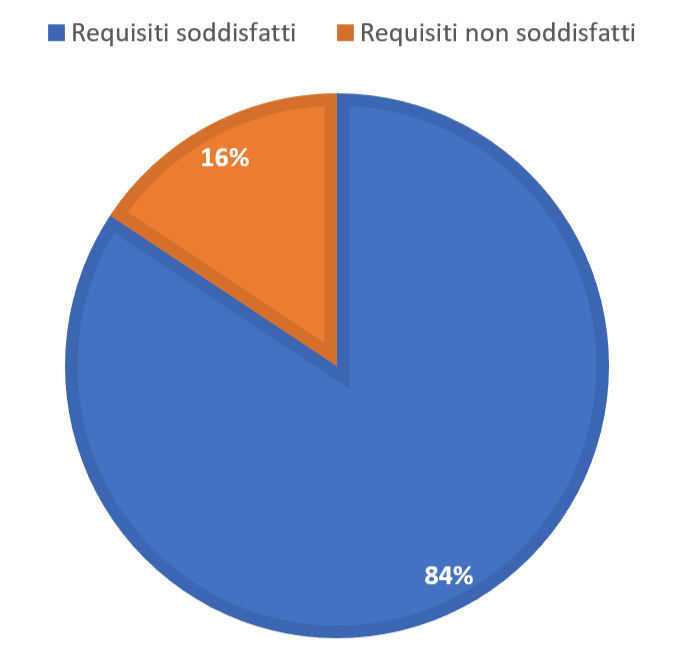
\includegraphics[width=7cm]{Images/RequisitiTotali}
\centering
\caption{Percentuale dei requisiti funzionali soddisfatti}
\end{figure}

Riguardo invece ai soli requisiti obbligatori la copertura ha raggiunto il 100\%, soddisfando quindi tutti i requisiti individuati.
\begin{figure}[hb]
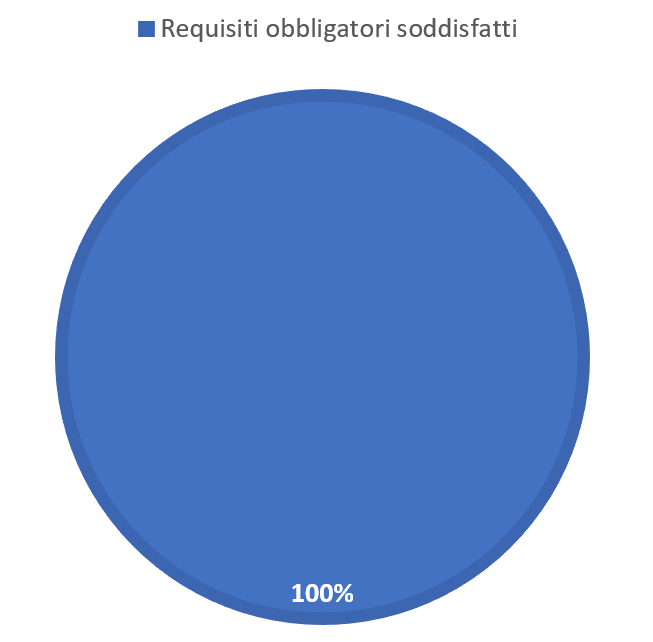
\includegraphics[width=7cm]{Images/RequisitiObbligatori}
\centering
\caption{Percentuale dei requisiti funzionali obbligatori soddisfatti}
\end{figure}